\documentclass[a4paper]{article}

%%%%%%%% CREATE DOCUMENT STRUCTURE %%%%%%%%
%% Language and font encodings
\usepackage[english]{babel}
\usepackage[utf8x]{inputenc}
\usepackage[T1]{fontenc}
%\usepackage{subfig}
\usepackage[table,xcdraw]{xcolor}

%% Sets page size and margins
\usepackage[a4paper,top=3cm,bottom=2cm,left=2cm,right=2cm,marginparwidth=1.75cm]{geometry}

%% Useful packages
\usepackage{enumitem}
\usepackage{amsmath}
\usepackage{amssymb}
\usepackage{graphicx}
\usepackage[colorinlistoftodos]{todonotes}
\usepackage[colorlinks=true, allcolors=blue]{hyperref}
\usepackage{caption}
\usepackage{subcaption}
\usepackage{multicol}
%\usepackage{sectsty}
%\usepackage{apacite}
\usepackage{float}
\usepackage{titling} 
\usepackage{blindtext}
\usepackage[square,sort,comma,numbers]{natbib}
\usepackage[colorinlistoftodos]{todonotes}
%\usepackage{xcolor}
\usepackage{indentfirst}
\usepackage{amsmath}
\usepackage[linesnumbered,algoruled,boxed,lined]{algorithm2e}
\setlength\parskip{.5\baselineskip plus .1\baselineskip  minus .1\baselineskip}
\setlength{\parindent}{1em}
\definecolor{darkgreen}{rgb}{0.0, 0.4, 0.0}

% \makeatletter
% \def\BState{\State\hskip-\ALG@thistlm}
% \makeatother


%%%%%%%% DOCUMENT %%%%%%%%
\begin{document}



%%%% Title Page
\begin{titlepage}

\newcommand{\HRule}{\rule{\linewidth}{0.5mm}} 							% horizontal line and its thickness
\newenvironment{bottompar}{\par\vspace*{\fill}}{\clearpage}
\center 
\begin{center}
%----------------------------------------------------------------------------------------
%	HEADING SECTIONS
%----------------------------------------------------------------------------------------

\includegraphics[scale=0.8]{./img/upclogo.png}\\[2cm] % Include a department/university logo - this will require the graphicx package
 
%\textsc{\LARGE Polytechnical University of Catalonia}\\[1cm] % Name of your university/college
\textsc{\Large Master in Innovation and Research in Informatics}\\[0.5cm] % Major heading such as course name
\textsc{\large Machine Learning}\\[5cm] % Minor heading such as course title

%----------------------------------------------------------------------------------------
%	TITLE SECTION
%----------------------------------------------------------------------------------------

\HRule \\[0.4cm]
{ \huge \bfseries House Price Prediction}\\[0.4cm] % Title of your document
\HRule \\[1.5cm]
 
%----------------------------------------------------------------------------------------
%	AUTHOR SECTION
%----------------------------------------------------------------------------------------
\begin{bottompar}
\begin{minipage}{0.5\textwidth}
\begin{flushleft} \large
\emph{Authors:}\\
Asaf Badouh \\ Pau Rodríguez Esmerats % Your name
\end{flushleft}
\end{minipage}
~
\begin{minipage}{0.4\textwidth}
\begin{flushright} \large
\emph{Professors:} \\
Jaume Baixeries Juvillà	\\ Marta Arias Vicente   % Supervisor's Name
\end{flushright}
\end{minipage}\\[2cm]

% If you don't want a supervisor, uncomment the two lines below and remove the section above
%\Large \emph{Author:}\\
%John \textsc{Smith}\\[3cm] % Your name

%----------------------------------------------------------------------------------------
%	DATE SECTION
%----------------------------------------------------------------------------------------

{\large \today}\\[2cm] % Date, change the \today to a set date if you want to be precise
\end{bottompar}
\end{center}
\end{titlepage}

\setcounter{tocdepth}{2}
\tableofcontents
\pagebreak

% \begin{abstract}


% \end{abstract}

\pagebreak


\section{Introduction}

% general purpose of the project
The goal of this project is to make the most out of data on house prices to build a model that is able to predict the price of a house based on it's attributes (Table\ref{table:dataFeatures}).
This includes pre-processing the data, performing feature engineering (feature selection and/or extraction) and training a regression model to predict the price. \\
An important part of our effort will be focused on the decision about what are the most important variables or features that we could extract upon them, as well as what are the best parameter configurations for the model we will train. Different approaches to each phase will be considered and compared appropriately before choosing the final implementation.

% organization of the report
This report is organized in different sections. First the different analysis approaches over the data are presented, where we discuss preprocessing, manual exploration, unsupervised analysis and testing assumptions over the data. Secondly, the different feature extraction techniques and resulting feature sets are explained. Then the different types of models and their configuration are presented. Finally, we explain the approach to perform feature selection and model selection throught different experiments. In the end, the conclusion of our work are presented.


\begin{table}[H]
\centering
\resizebox{\textwidth}{!}{
\begin{tabular}{lll}
\hline
\rowcolor[HTML]{C0C0C0} 
id             & a notation for a house                                                                                                                                 & Numeric \\
date           & Date house was sold                                                                                                                                    & String  \\
\rowcolor[HTML]{C0C0C0} 
price          & Price is prediction target                                                                                                                             & Numeric \\
bedrooms       & Number of Bedrooms/House                                                                                                                               & Numeric \\
\rowcolor[HTML]{C0C0C0} 
bathrooms      & Number of bathrooms/bedrooms                                                                                                                           & Numeric \\
sqft\_living   & square footage of the home                                                                                                                             & Numeric \\
\rowcolor[HTML]{C0C0C0} 
sqft\_lot      & square footage of the lot                                                                                                                              & Numeric \\
floors         & Total floors (levels) in house                                                                                                                         & Numeric \\
\rowcolor[HTML]{C0C0C0} 
waterfront     & House which has a view to a waterfront                                                                                                                 & Numeric \\
view           & Has been viewed                                                                                                                                        & Numeric \\
\rowcolor[HTML]{C0C0C0} 
condition      & How good the condition is ( Overall )                                                                                                                  & Numeric \\
grade          & \begin{tabular}[c]{@{}l@{}}overall grade given to the housing unit, \\ based on King County grading system\end{tabular}                                & Numeric \\
\rowcolor[HTML]{C0C0C0} 
sqft\_above    & square footage of house apart from basement                                                                                                            & Numeric \\
sqft\_basement & square footage of the basement                                                                                                                         & Numeric \\
\rowcolor[HTML]{C0C0C0} 
yr\_built      & Built Year                                                                                                                                             & Numeric \\
yr\_renovated  & Year when house was renovated                                                                                                                          & Numeric \\
\rowcolor[HTML]{C0C0C0} 
zipcode        & zip                                                                                                                                                    & Numeric \\
lat            & Latitude coordinate                                                                                                                                    & Numeric \\
\rowcolor[HTML]{C0C0C0} 
long           & Longitude coordinate                                                                                                                                   & Numeric \\
sqft\_living15 & \begin{tabular}[c]{@{}l@{}}Living room area in 2015(implies-- some renovations) \\ This might or might not have affected the lotsize area\end{tabular} & Numeric \\
\rowcolor[HTML]{C0C0C0} 
sqft\_lot15    & lotSize area in 2015(implies-- some renovations)                                                                                                       & Numeric \\ \hline
\end{tabular}%
}
\caption{Dataset's features - House sales in king county}
\label{table:dataFeatures}
\end{table}


\section{Multivariate data analysis}

\subsection{Preprocessing}

\textbf{Missing data and Errors - } We inspect our dataset to find missing data (blanks\textbackslash Na's) or error values (e.g. negative numbers of rooms). Luckily our data is complete and we didn't need to handle and missing values.

\textbf{Outliers - } To determine if there are outliers on the data set, we will use the Robustified Mahalanobis distance  iterative algorithm (fig.\ref{mahalanobis}) from the Moutlier library function. To that purpose, we first filter out the categorical variables of the dataset and then feed the resulting data set into the algorithm. The results are the individuals sorted by their distance to the centroid. Our conlusion is that the first 8 individuals in that ordering are outliers. We remove them from the dataset.



\begin{figure}[H]
\minipage{0.5\textwidth}%
    \centering
        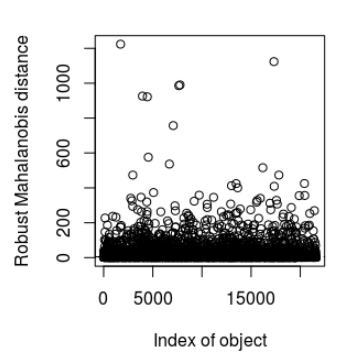
\includegraphics[width=0.7\textwidth]{img/mahalanobis.png}
    \caption{Robustified Mahalanobis distance for outliers detection }\label{mahalanobis}
\endminipage\hfill
\minipage{0.5\textwidth}%
    \centering
        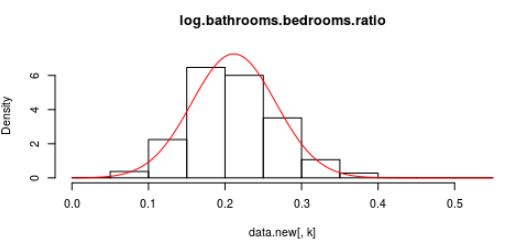
\includegraphics[width=0.9\textwidth]{img/gauss01.png}
    \caption{Plot of the histogram of a variable with a Normal distribution with same mean and variance }\label{gauss01}
\endminipage
\end{figure}
\vspace*{-15pt}

\subsection{Exploratory data analysis}
Briefly looking in the dataset's features (Table.\ref{table:dataFeatures}) we can see that not all features are useful for our work. We removed "id" and "date" from our table. The unique ID of individual is meaningless. Since we don't do time series analysis the date of sale is also useless. More details about feature extraction will be explained later.

\textbf{Histograms}

We start by ploting histograms of different variables of the dataset. With those we can start to estimate if data is far from normally distributed, if variables are from one or more than one process(fig.\ref{gauss01}).





\textbf{Plots}

We can also plot variables of the dataset by pairs, in order to appreciate which variables seem to be more correlated. 
We start by ploting variables with respect of the target (house price).

\begin{figure}[H]
    \centering
        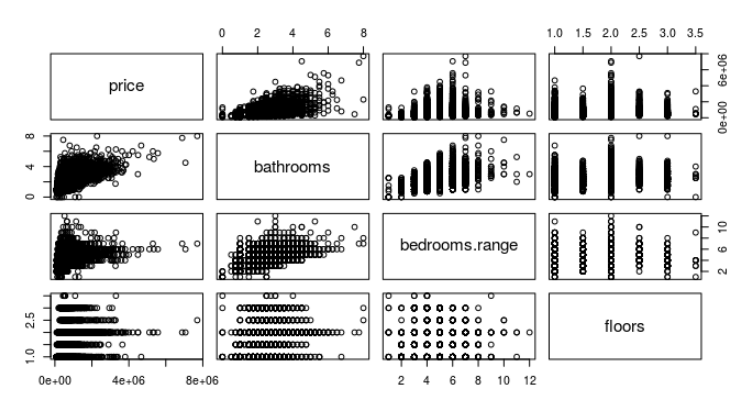
\includegraphics[width=0.8\textwidth]{img/pairs01.png}
    \caption{Plot of different variables against the price }\label{fig:rf_sfs}
\end{figure}

We expect to have some correlation based on the plots.

\textbf{Logarithm and ratio transformations}

We also explored how applying a logarithm to a variable or creating a ratio between 2 variables would affect the apparent correlation of the new variable with the target (house price):
\begin{figure}[H]
    \centering
        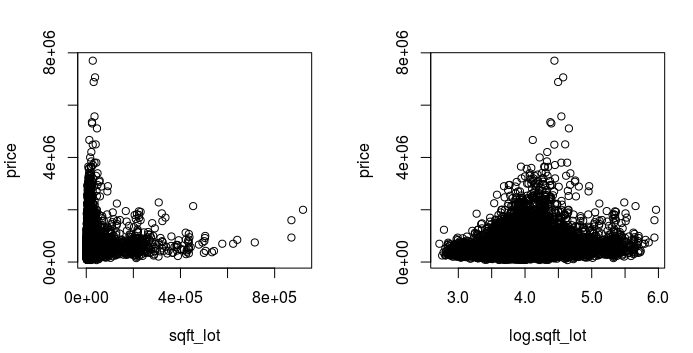
\includegraphics[width=0.8\textwidth]{img/log02.png}
    \caption{Plot the effect of the logarithm transformation }\label{fig:rf_sfs}
\end{figure}

We then decided to create some features that contain those transformations. (See section 3)

\textbf{Gaussianization}

It is important to know if the variables of the dataset are far or close to normality, in order to use some models that depend on the normality assumption(fig.\ref{gauss01}).

This is just approximate, but in case we find variables that deviate a from normality we can try to transform variables into a Gaussian version using the Box-Cox transform.

\begin{figure}[H]
    \centering
        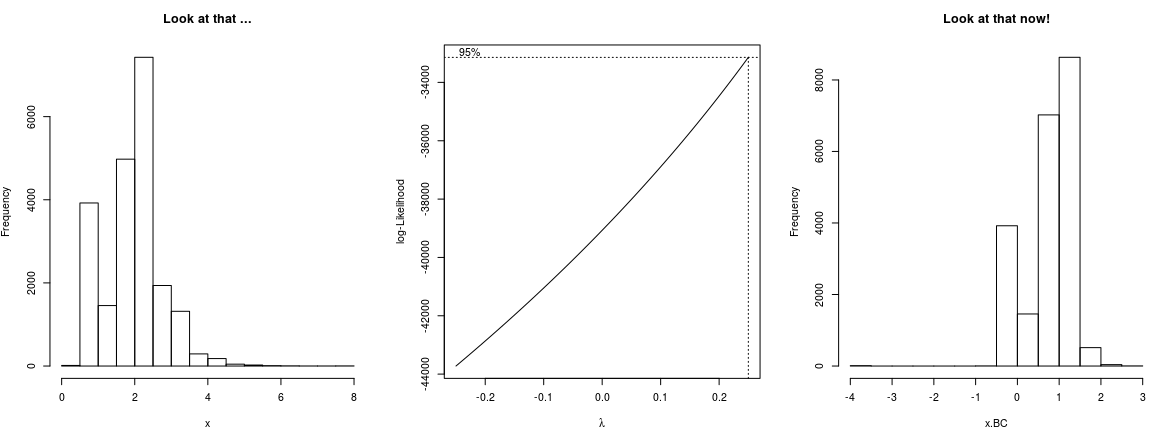
\includegraphics[width=0.8\textwidth]{img/Gauss03.png}
    \caption{Box-Cox transform for Gaussianization of a variable }\label{fig:rf_sfs}
\end{figure}

After trying some of those, it does not seem possible to Guassianize the variables of this dataset.


\subsection{Unsupervised analysis}


\begin{multicols}{2}

\textbf{PCA} In order to find some structure in the data we run PCA, as we can see in Figure.\ref{fig:PCA} there are strong correlation with many of the variable in the data set to our target (price variable). We learn that the area of living, the grade given by the city and number of bedrooms and bathrooms are important to when we want to analyze the price. On the other hand, the size of the basement and the properly size are not that important. 

\begin{figure}[H]
\centering
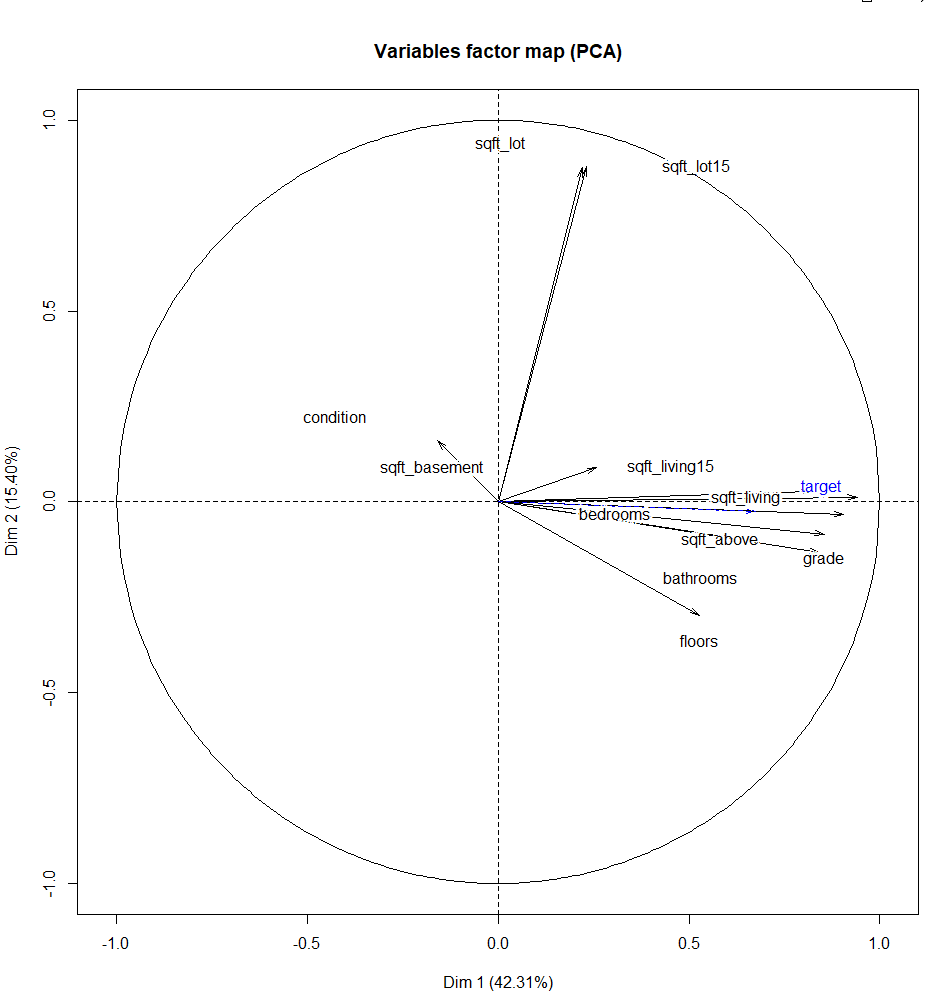
\includegraphics[width=0.49\textwidth]{img/PCA.png}
\caption{PCA}
\label{fig:PCA}
\end{figure}

\textbf{Clustering}
We clustered the individuals using hierarchical clustering. We did it using only continuous variables in order to see if we have some pattern in the data. As we can see in Fig.\ref{fig:hcluster}, more than $85\%$ of the individuals are grouped in a single cluster, the rest are divided into 2-3 clusters with smaller size. therefore, we deduce that we will not split our data into cluster and we will explore it as a whole.
% In case we will have time we would like to write something about the clustring using the projected individuals using PCA.
\begin{figure}[H]
\centering
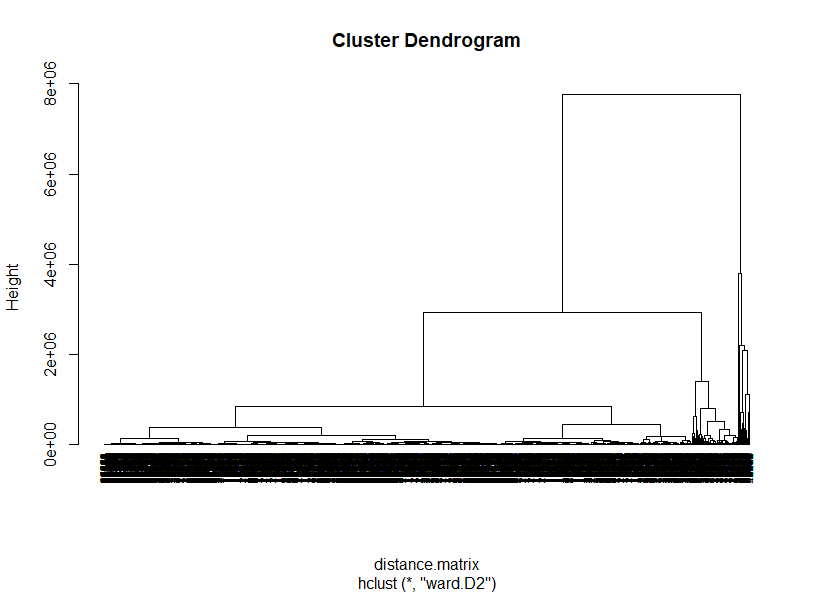
\includegraphics[width=0.48\textwidth]{img/Hclustering.png}
\caption{Hierarchical Clustering}
\label{fig:hcluster}
\end{figure}
\end{multicols}





\section{Feature extraction}

To improve the performance of the models that we want to train, we will explore some transformations of the initial dataset. We do that by extracting subsets of the variables, by applying transformations to them, by remove the variables that show more correlation or by creating a new dataset based on a principal components analysis.

\subsection{Intuitive transformations}

After the exploratory data analysis of section 1, we feel that transforming some variables with functions and trying different combinations can have an impact in terms of make the underlying structure of the data more accessible.

\textbf{Logs}

In the exploratory analysis we saw that applying the logarithm to some variables greatly changes they aspect when ploting them with the price target variable. We then decide to apply logarithms to some of the variables: bathrooms, bedrooms, sqft\_living, floors, sqft\_lot.



\textbf{Ratios}\\
While exploring the variables in our dataset we had the intuition about the ratio relationship between some variables. For example, the ratio between number of bedrooms to number of bathroom may be a good feature to help us predict the house price. Exploring on the Tax policy in USA\cite{tax}, we learn that tax of house also base on the characteristics of the house. Therefore we though it will be useful to check those features. We created new features based on ratios of pairs of the following list of variables from the dataset: bathrooms, bedrooms, sqft\_living, floors, sqft\_lot, logbathrooms, logbedrooms, logsqft\_living.


%"bathrooms.bedrooms.ratio"   "bedrooms.sqft.living.ratio" "bathroom.sqft.living.ratio" "sqft.ratio" "floor.sqft.living.ratio"   "floor.sqft.lot.ratio" "floor.bedrooms.ratio"       "floor.bathrooms.ratio"      "sqft.living.floors.ratio"  "bedrooms.floors.ratio"    



\subsection{Correlation}

Finally, we inspect different groups of variables to see which of them are highly correlated (a correlation greater than 0.7). We know a many machine learning models suffer from being trained over highly correlated variables. So we create new datasets based on subsets of features that are not highly correlated.

\begin{figure}[H]
    \centering
        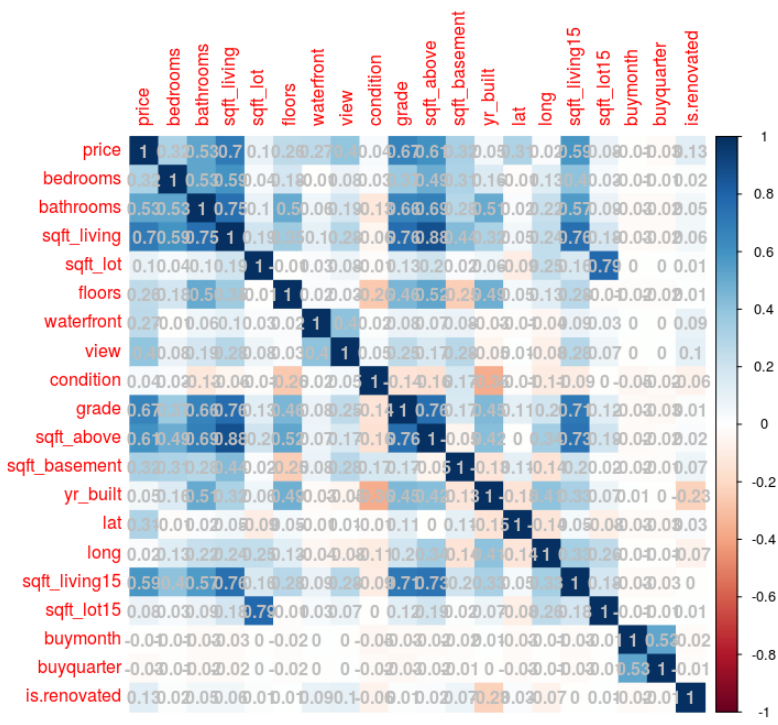
\includegraphics[width=0.8\textwidth]{img/corr01.png}
    \caption{Correlation matrix of a subset of tha continuous variables of the original dataset }\label{fig:rf_sfs}
\end{figure}
% plots

Based on that, we built 4 different subsets of features, where in each of them we will make sure that no pair of variables has a correlation higher than 0.7 or lower than -0.7. Two sets contain only different subsets of the original continuous variables with high correlations removed. Then a third subset contains logarithimic transformations with high correlations removed. Finally a fourth dataset contains ratio variables with high correlations removed. In each of them we remove one of the variables that is highly correlated with another one.

% lsit of subsets


\subsection{PCA}



\section{Models}

In this section we will present the different types of models that we will later train during the experiments. 

\subsection{Methodology}
% how did we proceed to select types of models to train
For the set of models that we chose to train in this project, we will apply the same methodology. First, the dataset over which we want to train the model will be split into a training and a testing set, by using random sampling with a proportion of 70\% individuals in the training and 30\% individuals in the testing set. Then the model will be trained over the training set by using k-fold cross validation, to select the best hyper parameter values for the model. After selecting the best hyper parameters, the model will be trained with those parameters over the whole training set. Finally, the trained model will be used to predict over the testing set to extract error measures and see how well the model generalizes.\\
In order to be able to compare over all the selected best models of each type, we will make sure that we extract the same error measure. In this case, we will use the normalized root mean squared error (NRMSE).

\subsection{Model types}
\textbf{Linear} We used the Linear model as the baseline to our exploration. This model has no control over the complexity so it is expected to overfit and perform worse than the other models overall.

\textbf{Ridge regression} This is one the most famous regularized linear models, using the L2 norm. It has a great support in libraries, with many implementations.

\textbf{Lasso regression}
This is another well-known regularized linear model, this one using the L1 norm. 

\textbf{PCR} This model is taking advantage of the PCA and use it to predict. First, the model will create PCA transformation over the training data, then we need to decide the number of PCs we want to use, we choose PCs' that will explain at least $90\%$ of the variance in the data. Later we predict using those PCs.

\textbf{Decision trees} We need to find tree that will give us good prediction but we don't want to have huge tree, therefore we needed to prune the tree using the complexity parameter. In first step we build a tree with cross-validation parameter of 10. Given full tree from the library we wish to prune it. We check the CV error of the best offer given tree (mostly it was the biggest tree the model created). To the CV error we added it's SD error, by that we get an interval of error for the best tree. Our next step is to choose the smallest tree that it's CV error is in that range. By prune the tree to that size we ensure that we will not have a complex tree and yet our CV error will be in the CV error range of the best tree this model can offer. One very important advantage of the tree is the ability to interpreted its decision. However,  since we don't do classification, it will get the centeroid of the leaf. In Figure.\ref{fig:dt},\ref{fig:dtp} we can see example of tree before and after pruning base on the initial dataset.

\begin{multicols}{2}
\begin{figure}[H]
\centering
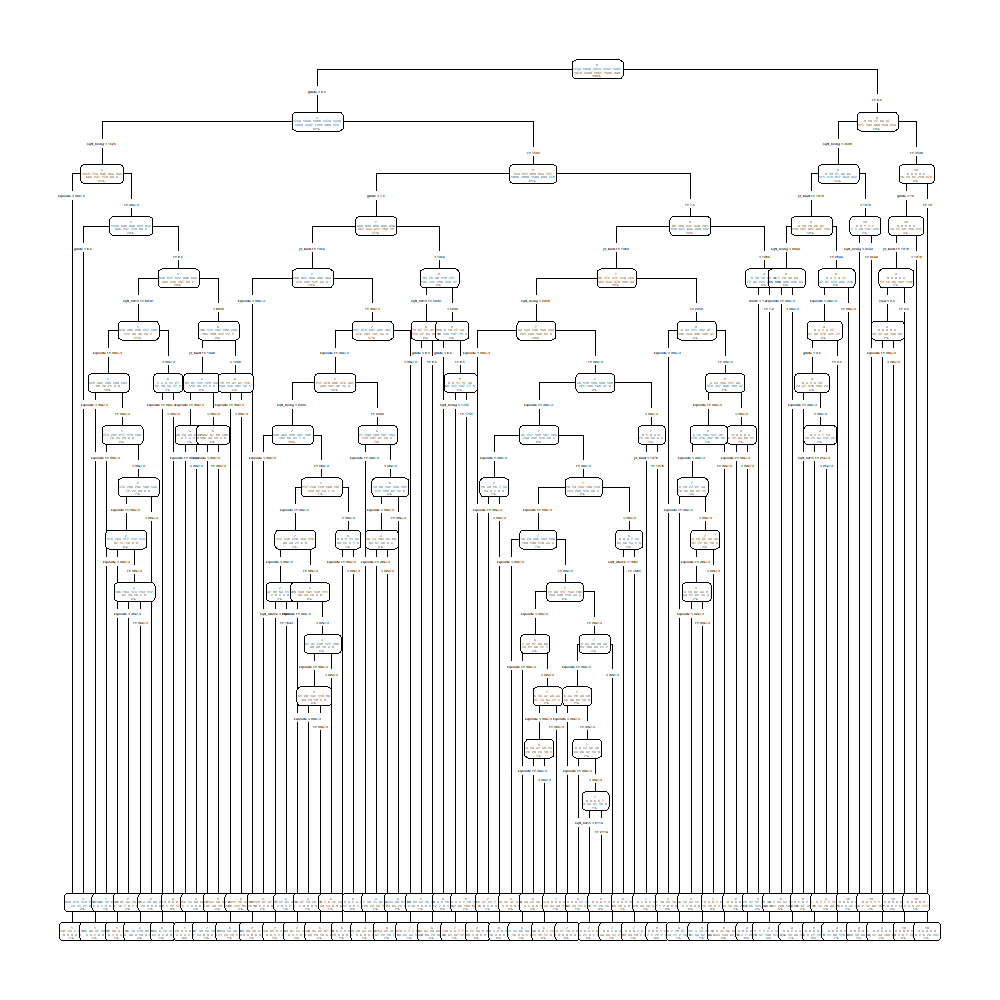
\includegraphics[width=0.48\textwidth]{img/trainingdt.png}
\caption{Full decision tree}
\label{fig:dt}
\end{figure}
\begin{figure}[H]
\centering
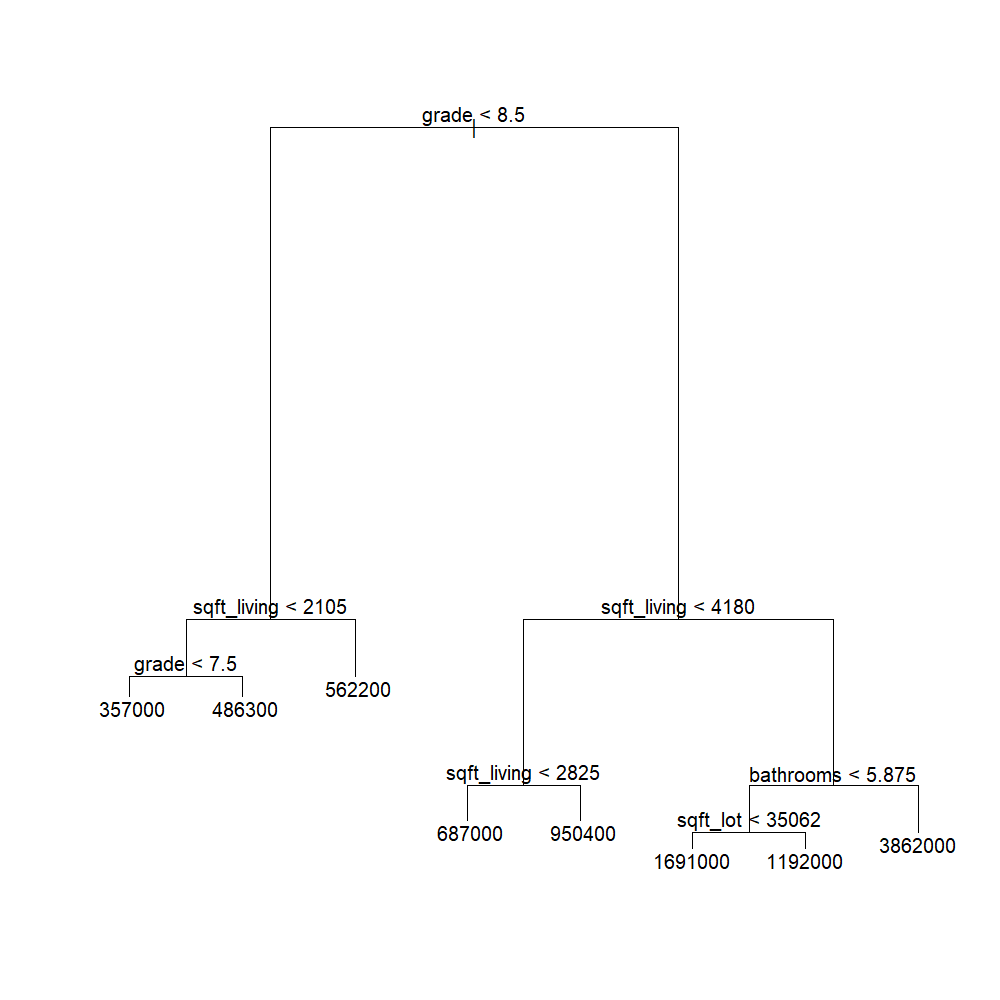
\includegraphics[width=0.48\textwidth]{img/regression_treelib_tree_training.png}
\caption{Prune decision tree}
\label{fig:dtp}
\end{figure}
\end{multicols}


\textbf{Random Forest} We need to find the optimum number of trees to generate. We do that using the MSE of the validatiion error. We train and validate number of models with over  different number of trees, then, we choose the model that have the minimum MSE. The next step was to train the model using the whole training data and predict. We use RandomForest R library.



\section{Experiments}

This section exposes the selected approach to perform feature and model selection through different experiments. An experiment consists on training a model over a selected dataset, using cross validation to select the hyper parameters that produce a model with the minimum validation error. Our strategy consists on explore the space of combinations of models and datatsets in order the find the best performing model over the best dataset. The steps we follow are summaryzed here:
\begin{itemize}
    \item First we start from a group of different datasets, each containing features produced on different analyses. 
    \item Then we train all the models that we have considered for the project over each of those datasets, performing cross validation each time.
    \item After that, we select the top 3 best pairs model-dataset, the ones with minimum validation error, and perform feature selection over the dataset using forward selection. 
    \item Finally, for each pair, the model is trained again over the resulting dataset.\\
\end{itemize}

The next table shows fragments of all the experiments and their error measures. For each experiment we printed the normalized root mean squared error obtained during the cross validation (shown as Validation.NRMSE), obtained as a mean of all the nrmse of each model and fold. This is the value that we use to select the best model, by selecting the minimum normalized root mean squared error. We also show the normalized mean squared error that the selected model, which is then trained again over all the training data set, obtains when predicting over the test set. This is the error that helps us see how well the selected model will generalize over new data.

\begin{figure}[H]
    \centering
        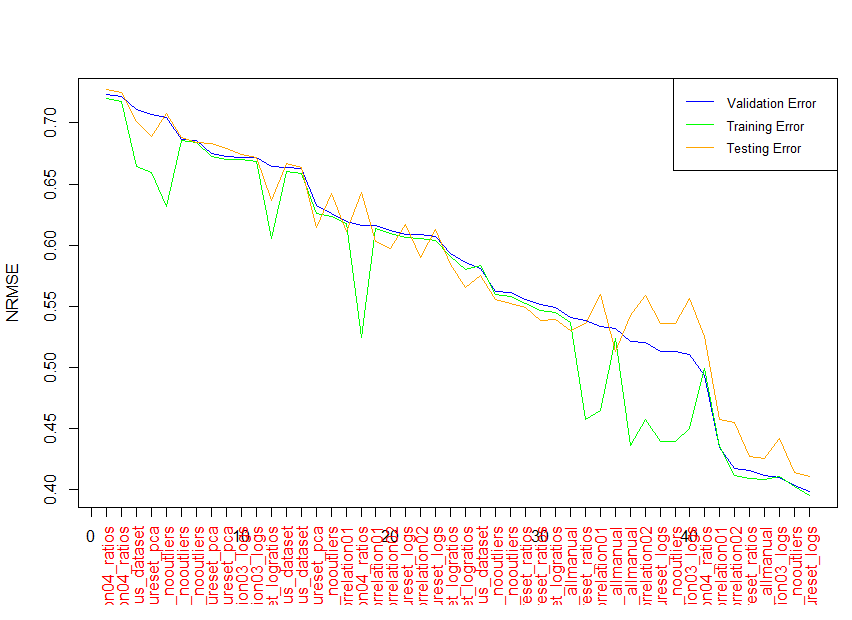
\includegraphics[width=0.95\linewidth]{img/exp01.png}
    \caption{Evolution of the NRMSE for the validation, training and testing set}\label{fig:Evol}
\end{figure}

% Summarized table
% latex table generated in R 3.4.3 by xtable 1.8-2 package
% 
\begin{table}[H]
\begin{tabular}{cllcc}
  \hline
 & subset[, 2] & Comment & Validation.NRMSE & Testing.NRMSE \\ 
  \hline
51 & regression\_randomforest & featureset\_logs & 0.40 & 0.41 \\ 
  56 & regression\_randomforest & featureset\_original\_nooutliers & 0.40 & 0.41 \\ 
  54 & regression\_randomforest & featureset\_nocorrelation03\_logs & 0.41 & 0.44 \\ 
  49 & regression\_randomforest & featureset\_allmanual & 0.41 & 0.43 \\ 
  59 & regression\_randomforest & featureset\_ratios & 0.42 & 0.43 \\ 
  53 & regression\_randomforest & featureset\_nocorrelation02 & 0.42 & 0.45 \\ 
  52 & regression\_randomforest & featureset\_nocorrelation01 & 0.43 & 0.46 \\ 
  55 & regression\_randomforest & featureset\_nocorrelation04\_ratios & 0.49 & 0.53 \\ 
  42 & regression\_tree\_rpartlib & featureset\_nocorrelation03\_logs & 0.51 & 0.56 \\ 
  39 & regression\_tree\_rpartlib & featureset\_logs & 0.51 & 0.54 \\ 
  44 & regression\_tree\_rpartlib & featureset\_original\_nooutliers & 0.51 & 0.54 \\ 
  41 & regression\_tree\_rpartlib & featureset\_nocorrelation02 & 0.52 & 0.56 \\ 
  37 & regression\_tree\_rpartlib & featureset\_allmanual & 0.52 & 0.54 \\ 
  25 & lasso regression GLMNET & featureset\_allmanual & 0.53 & 0.51 \\ 
  40 & regression\_tree\_rpartlib & featureset\_nocorrelation01 & 0.53 & 0.56 \\ 
  47 & regression\_tree\_rpartlib & featureset\_ratios & 0.54 & 0.54 \\ 
  13 & ridge regression GLMNET & featureset\_allmanual & 0.54 & 0.53 \\ 
  50 & regression\_randomforest & featureset\_logratios & 0.55 & 0.54 \\ 
  35 & lasso regression GLMNET & featureset\_ratios & 0.55 & 0.54 \\ 
  23 & ridge regression GLMNET & featureset\_ratios & 0.56 & 0.55 \\ 
  32 & lasso regression GLMNET & featureset\_original\_nooutliers & 0.56 & 0.55 \\ 
  20 & ridge regression GLMNET & featureset\_original\_nooutliers & 0.56 & 0.56 \\ 
  60 & regression\_randomforest & raw\_continuous\_dataset & 0.58 & 0.58 \\ 
  26 & lasso regression GLMNET & featureset\_logratios & 0.59 & 0.57 \\ 
  14 & ridge regression GLMNET & featureset\_logratios & 0.59 & 0.58 \\ 
  27 & lasso regression GLMNET & featureset\_logs & 0.61 & 0.61 \\ 
  29 & lasso regression GLMNET & featureset\_nocorrelation02 & 0.61 & 0.59 \\ 
  15 & ridge regression GLMNET & featureset\_logs & 0.61 & 0.62 \\ 
  17 & ridge regression GLMNET & featureset\_nocorrelation02 & 0.61 & 0.60 \\ 
  28 & lasso regression GLMNET & featureset\_nocorrelation01 & 0.62 & 0.60 \\ 
  43 & regression\_tree\_rpartlib & featureset\_nocorrelation04\_ratios & 0.62 & 0.64 \\ 
  16 & ridge regression GLMNET & featureset\_nocorrelation01 & 0.62 & 0.61 \\ 
  57 & regression\_randomforest & featureset\_pca\_nooutliers & 0.63 & 0.64 \\ 
  58 & regression\_randomforest & featureset\_pca & 0.63 & 0.61 \\ 
  36 & lasso regression GLMNET & raw\_continuous\_dataset & 0.66 & 0.66 \\ 
  24 & ridge regression GLMNET & raw\_continuous\_dataset & 0.66 & 0.67 \\ 
  38 & regression\_tree\_rpartlib & featureset\_logratios & 0.66 & 0.64 \\ 
  30 & lasso regression GLMNET & featureset\_nocorrelation03\_logs & 0.67 & 0.67 \\ 
  18 & ridge regression GLMNET & featureset\_nocorrelation03\_logs & 0.67 & 0.67 \\ 
  34 & lasso regression GLMNET & featureset\_pca & 0.67 & 0.68 \\ 
  22 & ridge regression GLMNET & featureset\_pca & 0.68 & 0.68 \\ 
  33 & lasso regression GLMNET & featureset\_pca\_nooutliers & 0.69 & 0.68 \\ 
  21 & ridge regression GLMNET & featureset\_pca\_nooutliers & 0.69 & 0.69 \\ 
  45 & regression\_tree\_rpartlib & featureset\_pca\_nooutliers & 0.70 & 0.71 \\ 
  46 & regression\_tree\_rpartlib & featureset\_pca & 0.71 & 0.69 \\ 
  48 & regression\_tree\_rpartlib & raw\_continuous\_dataset & 0.71 & 0.70 \\ 
  31 & lasso regression GLMNET & featureset\_nocorrelation04\_ratios & 0.72 & 0.72 \\ 
  19 & ridge regression GLMNET & featureset\_nocorrelation04\_ratios & 0.72 & 0.73 \\ 

   \hline
\end{tabular}
\label{experiments}\caption{Experiments performed and their NRMSE for validation and testing }

\end{table}

We also show in the fig.\ref{fig:Evol} how the mean of the normalized root mean squared error (NRMSE) when performing cross validation evolves in the different datasets, and compare it to how the training and test NRMSE performs.






% top 3 table
Our top 3 best performers consists of Random forest, Decision tree and Lasso regression models trained over feature datasets that contains logarithms of continuous variables, manually selected continuous vars that are not correlated between them or all the original dataset.
% latex table generated in R 3.4.3 by xtable 1.8-2 package
% 
\begin{table}[H]
\begin{tabular}{cllcc}
  \hline
 & Model & Dataset & Validation NRMSE & Testing NRMSE \\ 
  \hline
  51 & regression\_randomforest & featureset\_logs & 0.40 & 0.41 \\ 
  42 & regression\_tree\_rpartlib & featureset\_nocorrelation03\_logs & 0.51 & 0.56 \\ 
  25 & lasso regression GLMNET & featureset\_allmanual & 0.53 & 0.51 \\ 
  
   \hline
\end{tabular}
\label{experiments}\caption{Experiments performed and their NRMSE for validation and testing }
\end{table}


% forward selection explanation
Once we have found our best performing model and datasets, we run a forward selection algorithm to perform feature selection over each dataset with its corresponding model.\\

% forward selection table

%\scalebox{0.8}{

\begin{table}[H]
\centering
\resizebox{0.75\textwidth}{!}{
\begin{tabular}{cllcc}
  \hline
 & Model & Feature set & Validation.NRMSE & Testing.NRMSE \\ 
  \hline
1 & regression\_randomforest & featureset\_logs & 1.00 & 1.00 \\ 
  2 & regression\_randomforest & featureset\_logs 1\_7\_8\_13 & 0.98 & 0.98 \\ 
  3 & regression\_randomforest & featureset\_logs 1\_7\_8\_14 & 0.96 & 0.96 \\ 
  4 & regression\_randomforest & featureset\_logs 1\_7\_8\_15 & 0.99 & 1.00 \\ 
  5 & regression\_randomforest & featureset\_logs 1\_7\_8\_16 & 0.74 & 0.75 \\ 
  6 & regression\_randomforest & featureset\_logs 1\_7\_8\_17 & 0.83 & 0.81 \\ 
  7 & regression\_randomforest & featureset\_logs 1\_7\_8\_18 & 0.95 & 0.94 \\ 
  8 & regression\_randomforest & featureset\_logs 1\_7\_8\_19 & 0.82 & 0.83 \\ 
  9 & regression\_randomforest & featureset\_logs 1\_7\_8\_20 & 0.97 & 0.97 \\ 
  10 & regression\_randomforest & featureset\_logs 1\_7\_8\_16\_13 & 0.73 & 0.76 \\ 
  11 & regression\_randomforest & featureset\_logs 1\_7\_8\_16\_14 & 0.74 & 0.76 \\ 
  12 & regression\_randomforest & featureset\_logs 1\_7\_8\_16\_15 & 0.73 & 0.74 \\ 
  13 & regression\_randomforest & featureset\_logs 1\_7\_8\_16\_17 & 0.72 & 0.71 \\ 
  14 & regression\_randomforest & featureset\_logs 1\_7\_8\_16\_18 & 0.70 & 0.71 \\ 
  15 & regression\_randomforest & featureset\_logs 1\_7\_8\_16\_19 & 0.71 & 0.72 \\ 
  16 & regression\_randomforest & featureset\_logs 1\_7\_8\_16\_20 & 0.72 & 0.75 \\ 
  17 & regression\_randomforest & featureset\_logs 1\_7\_8\_16\_18\_13 & 0.70 & 0.71 \\ 
  18 & regression\_randomforest & featureset\_logs 1\_7\_8\_16\_18\_14 & 0.71 & 0.71 \\ 
  19 & regression\_randomforest & featureset\_logs 1\_7\_8\_16\_18\_15 & 0.71 & 0.73 \\ 
  20 & regression\_randomforest & featureset\_logs 1\_7\_8\_16\_18\_17 & 0.67 & 0.67 \\ 
  21 & regression\_randomforest & featureset\_logs 1\_7\_8\_16\_18\_19 & 0.69 & 0.69 \\ 
  22 & regression\_randomforest & featureset\_logs 1\_7\_8\_16\_18\_20 & 0.69 & 0.71 \\ 
  23 & regression\_randomforest & featureset\_logs 1\_7\_8\_16\_18\_17\_13 & 0.64 & 0.64 \\ 
  24 & regression\_randomforest & featureset\_logs 1\_7\_8\_16\_18\_17\_14 & 0.66 & 0.65 \\ 
  25 & regression\_randomforest & featureset\_logs 1\_7\_8\_16\_18\_17\_15 & 0.65 & 0.64 \\ 
  26 & regression\_randomforest & featureset\_logs 1\_7\_8\_16\_18\_17\_19 & 0.66 & 0.65 \\ 
  27 & regression\_randomforest & featureset\_logs 1\_7\_8\_16\_18\_17\_20 & 0.64 & 0.63 \\ 
  28 & regression\_randomforest & featureset\_logs 1\_7\_8\_16\_18\_17\_13\_14 & 0.63 & 0.63 \\ 
  29 & regression\_randomforest & featureset\_logs 1\_7\_8\_16\_18\_17\_13\_15 & 0.63 & 0.62 \\ 
  30 & regression\_randomforest & featureset\_logs 1\_7\_8\_16\_18\_17\_13\_19 & 0.63 & 0.62 \\ 
  31 & regression\_randomforest & featureset\_logs 1\_7\_8\_16\_18\_17\_13\_20 & 0.63 & 0.63 \\ 
  32 & regression\_randomforest & featureset\_logs 1\_7\_8\_16\_18\_17\_13\_15\_14 & 0.62 & 0.62 \\ 
  33 & regression\_randomforest & featureset\_logs 1\_7\_8\_16\_18\_17\_13\_15\_19 & 0.61 & 0.61 \\ 
  34 & regression\_randomforest & featureset\_logs 1\_7\_8\_16\_18\_17\_13\_15\_20 & 0.62 & 0.62 \\ 
  35 & regression\_randomforest & featureset\_logs 1\_7\_8\_16\_18\_17\_13\_15\_19\_14 & 0.60 & 0.60 \\ 
  36 & regression\_randomforest & featureset\_logs 1\_7\_8\_16\_18\_17\_13\_15\_19\_20 & 0.60 & 0.60 \\ 
  37 & regression\_randomforest & featureset\_logs 1\_7\_8\_16\_18\_17\_13\_15\_19\_20\_14 & 0.59 & 0.59 \\ 
   \hline

\end{tabular}

}
\caption{Execution of the forward selection algorithm }
\label{table:sfsranfomforest}
\end{table}
%}

In this table we can observe how we add features to the dataset until the validation error stops decreasing. At that point the best feature set is found. We can plot the evolution of the error measure (NRMSE of the cross validation) during the execution of the forward selection algorithm. In Figure.\ref{fig:rf_sfs} We can see the error in each iteration space (between the dashed-orange-lines), in every iteration we choose the feature that decrease the error the most.


\begin{figure}[H]
    \centering
        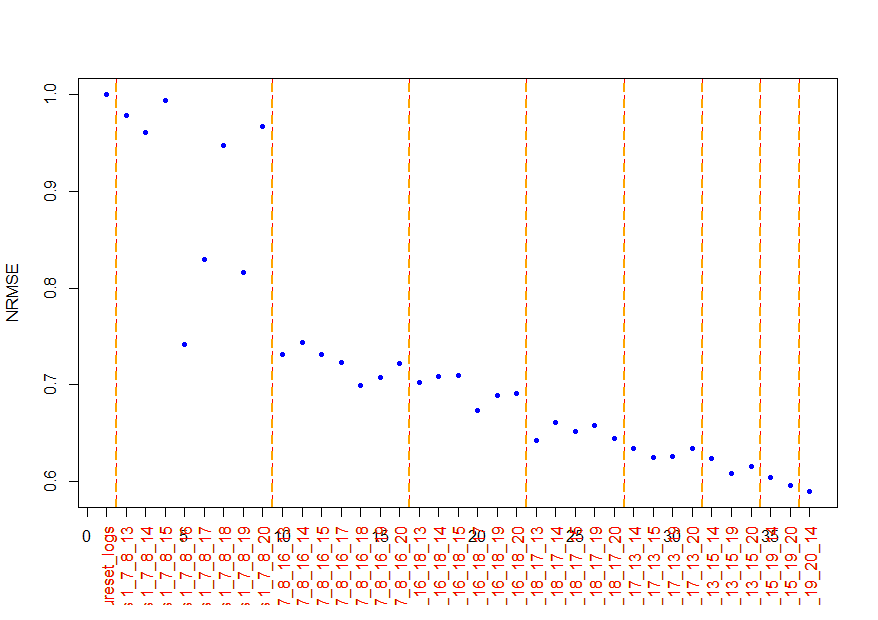
\includegraphics[width=0.8\textwidth]{img/randomForest.png}
    \caption{Evolution of the NRMSE for the Sequential forward selection}\label{fig:rf_sfs}
\end{figure}

We used SFS on the two best models, decision tree and lasso.
\textbf{Decision tree} - Using feature-set without correlated features gives us good results, knowing how decision tree this can be explained by the fact that every split will try to maximize the differences between it's nodes. When we are using features that are not correlate with each other it should help the model do better in it's splitting decision. We start the SFS with 8 features and add features iteratively. Eventually, the validation error dropped from 0.66 to 0.51.
\textbf{Lasso} - We used dataset with large range of features we extract. Start with the small number of features having validation error of 0.68, after 351 iteration of SFS algorithm, the final number of feature grow significantly and so the validation error dropped to 0.54.


%\scalebox{0.8}{
%% latex table generated in R 3.4.3 by xtable 1.8-2 package
% 
\begin{tabular}{cllcc}
  \hline
 & Model & Feature set & Validation.NRMSE & Testing.NRMSE \\ 
  \hline
1 & regression\_tree\_rpartlib & featureset\_nocorrelation03\_logs & 0.66 & 0.69 \\ 
  & ... & & ...& ... \\ 
  16 & regression\_tree\_rpartlib & featureset\_nocorrelation03\_logs 1\_2\_3\_4\_5\_6\_7\_8 & 0.51 & 0.56 \\ 
  & & \_10\_13\_9\_12\_11 & & \\
   \hline
\end{tabular}



%}\\
%\textbf{Forward selection of the decision tree model over the "featureset\_nocorrelation03\_logs" dataset:}\\


%\scalebox{0.8}{
%% latex table generated in R 3.4.3 by xtable 1.8-2 package
% 

\begin{tabular}{cllcc}
  \hline
 & Model & Feature set & Validation.NRMSE & Testing.NRMSE \\ 
  \hline
1 & lasso regression GLMNET & featureset\_allmanual & 0.68 & 0.66 \\ 
  2 & lasso regression GLMNET & featureset\_allmanual 1\_2\_3\_4\_5\_6\_7\_8\_9 & 0.68 & 0.65 \\ 
  & ... & & ... & ...\\
  351 & lasso regression GLMNET & featureset\_allmanual 1\_2\_3\_4\_5\_6 & 0.54 & 0.52 \\
   &  & \_7\_8\_16\_10\_13\_26\_28\_15\_30\_17\_18\_9 &  & \\ 
    &  & \_34\_20\_32\_35\_21\_14\_27\_19\_24\_33 &  & \\ 
   \hline
\end{tabular}


%}\\
%\textbf{Forward selection of the lasso model over the "featureset\_nocorrelation03\_logs" dataset:}\\


% forward selection plot




% explanation of the final fit
Once we have selected our best 3 models and performed feature selection over the dataset, we can fit the best model with the feature set and see what is its validation error and how it generalizes by the testing error.

% small resulting table of the final validatio errors




\section{Conclusion}

% important points to highlight
%   1- data analysis
%   2- feature extraction
%   3- model training
%   4- feature selection and model selection
We start with manual data exploration  using unsupervised techniques, checking for outliers and structures in the dataset. In the next step we did feature engineering for creating new features using ratio, log and other transformations. Facing the million dollar question which combination of feature set and model is the best for our problem, we decided to implement sequential forward selection. After many steps trail and error, we came up with the results in Table.\ref{table:final}. The most interesting to see, in our point of view, is the comparison between the decision tree and the Random forest. As we can see in the decision tree preform better than random tree. However, this is base on the subset we used from SFS, looking on Table.\ref{experiments} we see that the Random forest model that trained with the complete data set (featureset\_logs) preform much better. But when we used SFS not all the features were chosen, that show us that doing SFS is good, but not enough. On the other hand, we see that the decision tree model didn't suffer from that, we assume it because it have less randomness in it's process. About the Lasso regression model, we expected it be worse than Random Forest, but using the best featureset (by forward selection) we found that this is not the case. This is a bit surprising, we can also say the difference is not so significant.

% 

% mentions the manual exploration and feature extraction
% metion the unsupervised analysis and pca feature extraction
% mention the methodology forward selection
% mention the results : which model outperforms the others 
% compare the models in the top 3
% state why random forest is better than decision trees and lasso -> theoretically should be easy to give reasons for that
% IMprovements: 


We proposed a series of improvements over the current work:
\begin{itemize}
    \item test more advanced models: Splines, RVM, Bayesian approach to regression,
    \item perform a deeper exploration of the possible features and combinations of features
    \item Explore better feature selection method.
\end{itemize}
\begin{table}[H]
\centering
\resizebox{\textwidth}{!}{
\begin{tabular}{cllccc}
  \hline
 & Model & Feature set & Validation.NRMSE & Training.NRMSE & Testing.NRMSE \\ 
  \hline
1 & regression\_tree\_rpartlib & featureset\_regression\_rpart\_tree\_fitting\_sfs & 0.51 & 0.45 & 0.56 \\ 
  2 & lasso regression GLMNET & featureset\_glmnet\_lasso\_sfs & 0.54 & 0.53 & 0.52 \\ 
  3 & regression\_randomforest & featureset\_regression\_randomforest\_sfs & 0.59 & 0.59 & 0.59 \\ 
   \hline
\end{tabular}
}
\caption{Best 3 models}
\label{table:final}
\end{table}


\newpage
\nocite{*}
\bibliographystyle{unsrt}
\bibliography{references}
\end{document}